\begin{figure}[H]
    \centering
    \resizebox{0.52\textwidth}{!}{%
    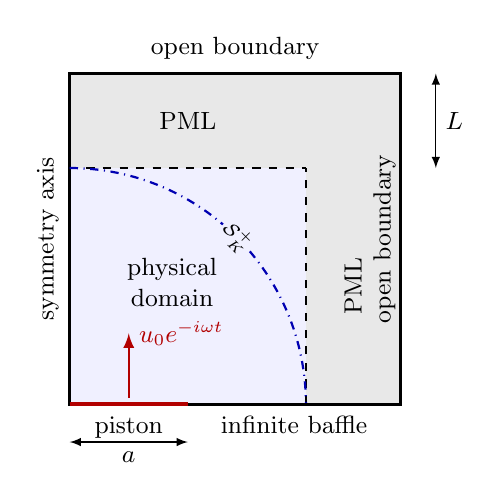
\begin{tikzpicture}[x=1cm,y=1cm,>=latex,font=\small]
        \def\inner{3.0}
        \def\outer{4.2}
        \def\piston{1.5}

        \fill[blue!6] (0,0) rectangle (\inner,\inner);
        \fill[gray!18] (\inner,0) rectangle (\outer,\outer);
        \fill[gray!18] (0,\inner) rectangle (\inner,\outer);
        \draw[very thick] (0,0) rectangle (\outer,\outer);
        \draw[dashed,thick] (\inner,0) -- (\inner,\inner);
        \draw[dashed,thick] (0,\inner) -- (\inner,\inner);
        \draw[dash dot,blue!70!black,thick]
            (0,\inner) arc[start angle=90,end angle=0,radius=\inner];

        \draw[red!70!black,line width=1.5pt] (0,0) -- (\piston,0);
        \draw[very thick] (\piston,0) -- (\outer,0);
        \draw[<->] (0,-0.48) -- (\piston,-0.48)
            node[midway,below] {$a$};
        \draw[->,red!70!black,thick] (0.75,0.08) -- (0.75,0.90)
            node[right] {$u_0e^{-i\omega t}$};

        \draw[<->] (4.65,\inner) -- (4.65,\outer)
            node[midway,right] {$L$};

        \node[rotate=90] at (-0.28,2.1) {symmetry axis};
        \node[align=center] at (1.3,1.55) {physical\\domain};
        \node[rotate=-45,fill=blue!6,inner sep=1pt,font=\scriptsize]
            at (2.12,2.12) {$\mathcal{S}_K^+$};
        \node[rotate=90] at (3.60,1.50) {PML};
        \node at (1.50,3.60) {PML};
        \node[below] at (0.75,-0.03) {piston};
        \node[below] at (2.85,-0.03) {infinite baffle};
        \node[above] at (2.1,{\outer+0.06}) {open boundary};
        \node[rotate=90,above] at ({\outer+0.06},2.1) {open boundary};
    \end{tikzpicture}
    }
    \caption{Axisymmetric baffled-piston configuration.  The rectangular PML
    occupies the outer radial and upper strips and their corner.  The
    dash-dotted arc is the upper Kirchhoff reconstruction auxiliary surface and not belong to any boundary.}
    \label{fig:pistonConfiguration}
\end{figure}
